\documentclass{article}
\usepackage[utf8]{inputenc}
\usepackage[left=1in,right=1in,top=1in,bottom=1in]{geometry}
\usepackage{crop,graphicx,array,color,flushend,stfloats,amsthm,chngpage,times,fancyhdr,lipsum,lastpage}

%%%%%%%%%%%%   Extra libraries & settings %%%%%%%%%%%%%
\setlength{\parskip}{0.25em}

%%%%%%%%%%%%   Header and Footer  %%%%%%%%%%%%%
\pagestyle{fancy}

\fancypagestyle{plain}{%
  \renewcommand{\headrulewidth}{0pt}%
  \fancyhf{}%
  \fancyfoot[R]{Page \bf\thepage\ \rm of \bf\pageref{LastPage}}%
}


%%%% Customise Titles and Headers: %%%%
\title{Don't forget adding title}
\author{Chinchuthakun Worameth (18B00033)}
\date{\today}

\fancyhf{}
\fancyhead[L]{Chinchuthakun Worameth}
\fancyhead[R]{18B00033}
\fancyfoot[R]{Page \bf\thepage\ \rm of \bf\pageref{LastPage}}


\AtBeginDocument{
%%%%%%%%%%%% Make Title and Format Lines %%%%%%%%%%%%
\maketitle											%
\vspace{-120px}										%
\noindent\rule{\linewidth}{1pt} \par				%
\vspace{100px}										%
\vspace{-20px}										%
\noindent\rule{\linewidth}{1pt} \par				%
\vspace{10px}										%
% %%%%%%%%%%%%%%%%%%% Content %%%%%%%%%%%%%%%%%%%%	
}

\AtEndDocument{
\bibliographystyle{IEEEtran}
\nocite{*}
\bibliography{citation}
}
% math stuff
\usepackage{amsmath}                % to use DeclareMathOperator
\usepackage{amssymb}
\usepackage{mathrsfs}
\usepackage{mathtools}
\usepackage{xargs}                  % for more than one optional arguments when define new commands
\usepackage{physics}                % vectors
\usepackage{mdframed}               % frames for definition, theorem, etc.
\usepackage[ruled]{algorithm2e}     % for algorithms
\usepackage{ifthen}                % for \ifthenelse
\usepackage{upgreek}

% figures and tables
\usepackage{titlesec}
\usepackage{caption}
\usepackage{subcaption}
\usepackage{multirow}
\usepackage{relsize}

% formatting some important single letters
\renewcommand{\epsilon}{\varepsilon}
\renewcommand{\phi}{\varphi}
\renewcommand{\upepsilon}{\upvarepsilon}
\renewcommand{\upphi}{\upvarphi}

% new operators
\DeclareMathOperator*{\argmin}{arg\,min}                % argmin
\DeclareMathOperator*{\argmax}{arg\,max}                % argmax
\DeclarePairedDelimiter\ceil{\lceil}{\rceil}            % ceiling function
\DeclarePairedDelimiter\floor{\lfloor}{\rfloor}         % floor function
\DeclarePairedDelimiter{\parens}{\lparen}{\rparen}      % parenthesis (use \parens* for automatically adjusting version)
\DeclarePairedDelimiter{\bracket}{[}{]}
\DeclarePairedDelimiter{\cbracket}{\{}{\}}
\DeclarePairedDelimiter{\ang}{\langle}{\rangle}
% \DeclarePairedDelimiter{\fourier}{\mathscr{F}\{}{\}}
% \DeclarePairedDelimiter{\invfourier}{\mathscr{F}^{-1}\{}{\}}

\newcommand{\fourier}[1]{\mathscr{F}\cbracket*{#1}}
\newcommand{\invfourier}[1]{\mathscr{F}^{-1}\cbracket*{#1}}
\newcommand {\dx}{\,dx}
\newcommand {\dy}{\,dy}
\newcommand {\dz}{\,dz}
\newcommand {\dt}{\,dt}
\newcommand {\du}{\,du}
\newcommand {\dtheta}{\,d\theta}
\newcommand {\domega}{\,d\omega}



\newcommand{\bigo}[1]{\ensuremath{\mathcal{O}\parens*{#1}}}
% new commands
\newcommand{\st}{such that }
\newcommand{\w}{where }
\newcommand{\del}{\nabla}
\newcommand{\larrow}{\leftarrow}
\newcommand{\rarrow}{\rightarrow}
\newcommand{\tbf}{\textbf}
\newcommand{\tit}{\textit}
\newcommand{\col}{\operatorname{col}}
\newcommand{\mat}[1]{\begin{matrix} #1 \end{matrix}}
% \newcommand{\vect}[1]{\boldsymbol{\mathbf{#1}}}
\newcommand{\vf}[1]{\boldsymbol{\mathbf{#1}}}
\newcommandx*{\seq}[2][1,2]{\ensuremath{#1, \ldots, #2}}
\newcommandx*{\ssum}[3][1,2,3]{\ensuremath{\sum_{#1 = #2}^{#3}}}
\newcommandx*{\sint}[2][1,2]{\ensuremath{\int_{#1}^{#2}}}
% \newcommandx*{\func}[4][1,2,3,4]{\ensuremath{#1^{\parens{#2}}_{#3}\parens{#4}}}
% \newcommandx*{\val}[3][1,2,3]{\ensuremath{#1^{\parens{#2}}_{#3}}}

% \newcommandx*{\func}[4][1=f,2=x,3,4, usedefault]{
%     \ifthenelse{\equal{#3}{}}{\ensuremath{#1_{#4}\parens{\vf{#2}}}}{\ensuremath{#1^{\parens{#3}}_{#4}\parens{\vf{#2}}}}
% }
\newcommandx*{\func}[3][1=f,2,3, usedefault]{
    \ifthenelse{\equal{#2}{}}{\ensuremath{#1_{#3}}}{\ensuremath{#1^{\parens{#2}}_{#3}}}
}
\newcommandx*{\val}[3][1,2,3, usedefault]{
    \ifthenelse{\equal{#2}{}}{\ensuremath{\vf{#1}_{#3}}}{\ensuremath{\vf{#1}^{\parens{#2}}_{#3}}}
}

\newcommandx*{\Real}[1][1, usedefault]{\ensuremath{\mathbb{R}^{#1}}}                % set of real number
\newcommandx*{\Int}[1][1, usedefault]{\ensuremath{\mathbb{Z}^{#1}}}                 % set of integer
\newcommandx*{\Natural}[1][1, usedefault]{\ensuremath{\mathbb{N}^{#1}}}             % set of natural number
\newcommandx*{\normal}[2][1=0, 2=1, usedefault=!]{\ensuremath{\mathcal{N}(#1,#2)}}  % Gaussian distribution

% define frame environment
% \newmdtheoremenv{definition}{Definition}
% \newmdtheoremenv{proposition}{Proposition}
% \newmdtheoremenv{corollary}{Corollary}
% \newmdtheoremenv{lemma}{Lemma}
% \newmdtheoremenv{theorem}{Theorem}
% \newmdtheoremenv{remark}{Remark}

% define keywords for algorithm
\SetKwInOut{Input}{Input}
\SetKwInOut{Output}{Output}
\SetKwInOut{Parameter}{Parameter}

% \begin{theorem}{text}{label}
% refer as \ref{tha:label}
\usepackage{tcolorbox}
\tcbuselibrary{theorems,breakable} %% を読み込む
\definecolor{burgundy}{rgb}{0.5, 0.0, 0.13}
\newtcbtheorem[number within=section]{theorem}{Theorem}%
{colframe=burgundy,colback=burgundy!2!white,
rightrule=0pt,leftrule=0pt,bottomrule=2pt,
colbacktitle=burgundy,theorem style=standard,breakable,arc=0pt}{theo}

\definecolor{oxfordblue}{rgb}{0.0, 0.13, 0.28}
\newtcbtheorem[number within=section]{definition}{Definition}%
{colframe=oxfordblue,colback=oxfordblue!2!white,
rightrule=0pt,leftrule=0pt,bottomrule=2pt,
colbacktitle=oxfordblue,theorem style=standard,breakable,arc=0pt}{def}

\definecolor{cadmiumorange}{rgb}{0.93, 0.53, 0.18}
\newtcbtheorem[number within=section]{remark}{Remark}%
{colframe=cadmiumorange,colback=cadmiumorange!2!white,
rightrule=0pt,leftrule=0pt,bottomrule=2pt,
colbacktitle=cadmiumorange,theorem style=standard,breakable,arc=0pt}{rem}

% equation numbering
\numberwithin{equation}{section}

%%%%%%%%%%%%%%%%%%%%%%%%%%%
\usepackage{listings}
\usepackage{xcolor}

\definecolor{codegreen}{rgb}{0,0.6,0}
\definecolor{codegray}{rgb}{0.5,0.5,0.5}
\definecolor{codepurple}{rgb}{0.58,0,0.82}
\definecolor{backcolour}{rgb}{0.95,0.95,0.92}

\lstdefinestyle{mystyle}{
    backgroundcolor=\color{backcolour},   
    commentstyle=\color{codegreen},
    keywordstyle=\color{magenta},
    numberstyle=\tiny\color{codegray},
    stringstyle=\color{codepurple},
    basicstyle=\ttfamily\footnotesize,
    breakatwhitespace=false,         
    breaklines=true,                 
    captionpos=b,                    
    keepspaces=true,                 
    numbers=left,                    
    numbersep=5pt,                  
    showspaces=false,                
    showstringspaces=false,
    showtabs=false,                  
    tabsize=2
}

\lstset{style=mystyle}

\makeatletter
\renewcommand*\env@matrix[1][\arraystretch]{%
  \edef\arraystretch{#1}%
  \hskip -\arraycolsep
  \let\@ifnextchar\new@ifnextchar
  \array{*\c@MaxMatrixCols c}}
\makeatother
\usepackage{subfiles}
\usepackage{subcaption}
\usepackage{hyperref}
\usepackage{CJKutf8}

\title{Computer Graphics Assignment \#7}
\begin{document}
\section{Question}
\begin{enumerate}
    \item Assuming that the scene is illuminated by a D65 light, render the top three primitive shapes with a texture of white chalk, a brick painted with a paint of the color of the \#74 pigment in the pigment data(pigments.zip), and copper metallic-like 10 yen coin from left to right. Report how to realize the characteristic of each material with your adopted algorithm, equations, coefficients, data, and screenshot images. ( The color matching functions for CIEXYZ1931 is XYZ\_CIE\_2.dat)
    
    \item Using the same light, render the bottom three primitive shapes with your favorite material textures and shader programs. The three chosen materials have to be different. Report the characteristics of the textures from the material point of view, and how to realize the material appearance with algorithms, equations, coefficients, data, and screenshot images.
\end{enumerate}

\begin{figure}[h]
    \centering
    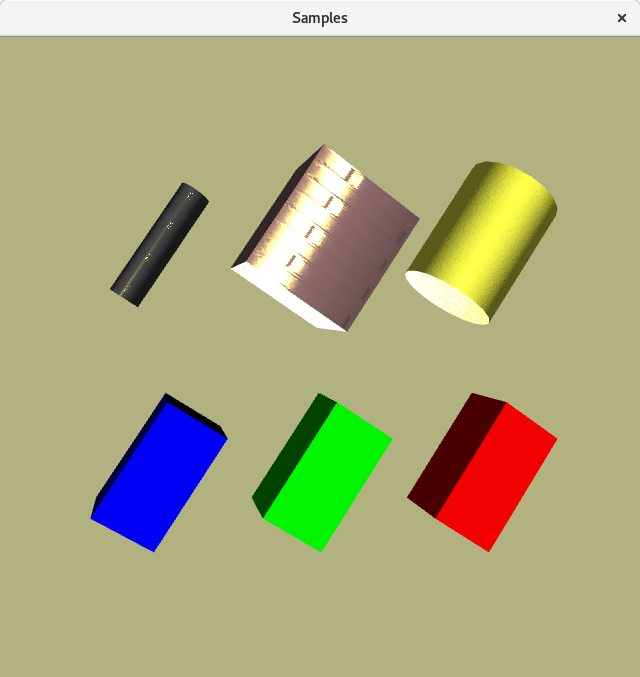
\includegraphics[width=0.6\textwidth]{figures/assignment7/assignment7-example.png}
    \caption{A screen shot of the program}
\end{figure}

\section{Answer}

This report is organized into 6 sections, ordered in the same way as the material displayed in Figure \ref{assignment7-snapshot}.

\subsection{White chalk}

The empirical reflection function can be described as
\begin{subequations} \label{empirical-reflection}
    \begin{gather}
        \val[H] = \frac{\val[L] + \val[V]}{2} \\
        \text{Dir} = K_d(\val[L] \cdot \val[N]) + K_s (\val[N] \cdot \val[H])^n \label{empirical-main}
    \end{gather}
\end{subequations}
where $\val[L]$, $\val[V]$, and $\val[N]$ are the incident light direction, the reflected light direction, and the surface normal, respectively. Note that the first and second term in Equation \eqref{empirical-main} represent diffuse reflection and specular reflection. 

Based on Equation \eqref{empirical-reflection}, we can model the reflected light on a white chalk texture as
\begin{subequations}\label{reflection-chalk}
    \begin{gather}
        \text{Diffuse} = K_d(\val[L] \cdot \val[N])(\val[C][][L] \odot \val[C][][R]) \\
        \text{Specular} = 0
    \end{gather}
\end{subequations}
where $\val[C][][L]$ and $\val[C][][R]$ are the 3-dimensional vectors representing RGB color coordinate of the incident light and the reflectant (material), respectively.

In the implementation, we use $K_d = 0.95, K_s = 8.5, n = 90.1$ in empirical reflection function. We employ a bump mapping to generate the white chalk texture from data available at \cite{texture-chalk}. Then, we initialize the color of material to be $(0.9095,0.9368,0.7559)$ in XYZ coordinate, which is converted from the RGB color data \cite{color-chalk} by using \cite{color-converter}. By implementing a shader program according to Equation \eqref{reflection-chalk}, we can create a realistic white chalk texture as shown on the next page.

\subsection{Brick}

Since bricks are made of material similar to white chalk, we also model the reflection by using Equation \eqref{reflection-chalk}. Similar to the previous material, we use a bump mapping to generate the brick texture from the data given together with the sample source codes. The XYZ coordinate color of the \#74 pigment is $(0.294606,0.480477,0.344893)$ as calculated in 
\href{https://colab.research.google.com/drive/1KD-4itGSez7aZ8Xvt2FDbf4bOZyQURiZ?usp=sharing}{\underline{the Assignment \#5}}.

\subsection{Copper}

Unlike the previous materials, copper is a metal; thus, having non-zero specular reflection. It can be described as
\begin{equation}\label{reflection-metal}
    \text{Specular} = K_s (\val[N] \cdot \val[H])^n (\val[C][][L] \odot \val[C][][R])
\end{equation}
We employ a bump mapping to generate the texture of copper from data available at \cite{texture-copper}. Then, we initialize the color of material to be $(0.2798,0.2316,0.0470)$ in XYZ coordinate, which is converted from the RGB color data \cite{color-copper} by using \cite{color-converter}. Finally, we implement a shader program according to Equation \eqref{reflection-metal}.

\subsection{Gold bar}

Similar to copper, gold is a metallic element; hence, can be modeled by using Equation \eqref{reflection-metal}. In the implementation, we use a bump mapping with texture available at \cite{texture-gold} and RGB color from \cite{color-gold}, which can be converted to $(0.6446,0.6293,0.0769)$ according to \cite{color-converter}.

\subsection{Plastic}

Unlike both chalk-like and metallic materials, plastic has specular reflection. However, the color from this type of reflection is not tinted by the color of the material itself. In other words, the specular reflection of plastic texture can be mathematically described as
\begin{equation}\label{reflection-plastic}
    \text{Specular} = K_s (\val[N] \cdot \val[H])^n \val[C][][L]
\end{equation}

To implement this texture, we use a bump mapping with texture available at \cite{texture-plastic} and RGB color from \cite{color-plastic}, which can be converted to $(0.4938,0.5336,0.3825)$ according to \cite{color-converter}.

\subsection{Wood}

Considering the material aspect, wood should not yield any specular reflection. However, to clearly illustrate the wood's texture in the program, we assume that the wood object has a layer of glossy lacquer; hence, having a specular reflection in a manner similar to plastic-like material. Therefore, we will use Equation \eqref{reflection-plastic} to model this material.

For the implementation, we use a bump mapping with texture available at \cite{texture-wood} and RGB color from \cite{color-wood} \footnote{Actually, the RGB coordinate in the reference is $(92,64,51)$. However, it cannot be properly rendered by using XYZ coordinate system, apparently. Therefore, we manually raised the value of $R$ to 150.}, which can be converted to $(0.1575,0.1066,0.0329)$ according to \cite{color-converter}.

%%% https://www.scratchapixel.com/lessons/3d-basic-rendering/phong-shader-BRDF

\begin{figure}[h]
    \centering
    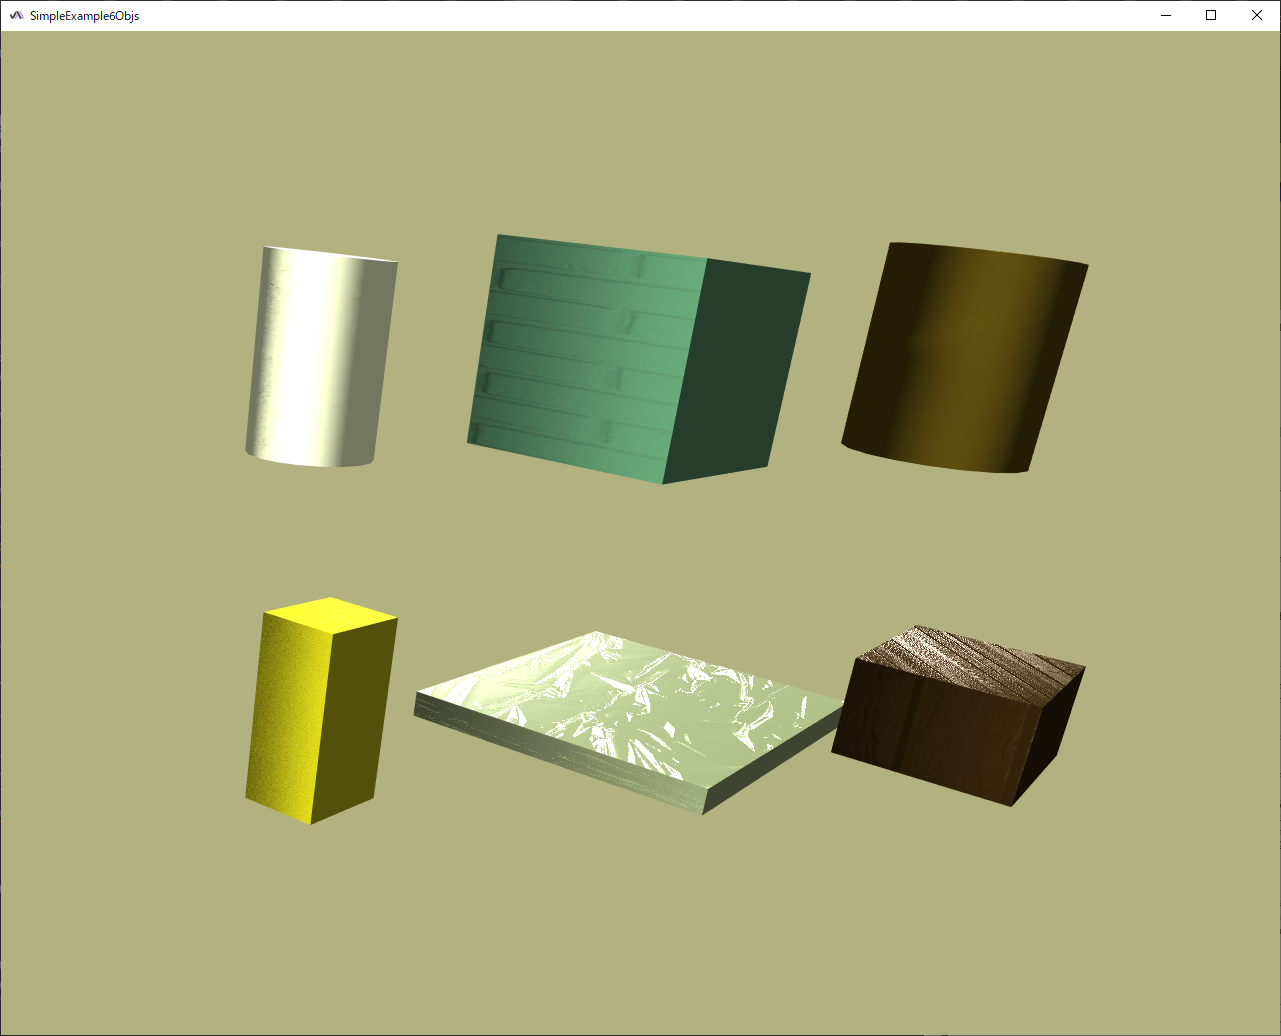
\includegraphics[width=0.7\textwidth]{figures/assignment7/assignment7-snapshot.png}
    \caption{A screen shot of the modified program. From left to right, top to bottom, the materials are: white chalk, brick with color of pigment \#74, copper, gold bar, plastic, and wood covered with lacquer}
    \label{assignment7-snapshot}
\end{figure}

\begin{CJK}{UTF8}{min}
    \bibliographystyle{IEEEtran}
    \bibliography{citation-assignment7}
\end{CJK}

\begin{figure}[htpb]
    \centering
    \subcaptionbox{White chalk \cite{texture-chalk}}{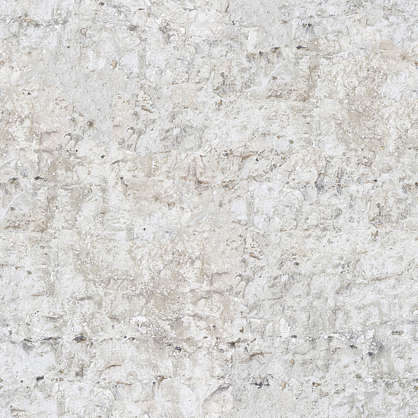
\includegraphics[width=0.3\textwidth]{figures/assignment7/white-chalk.png}}
    \hfill
    \subcaptionbox{Brick (given)}{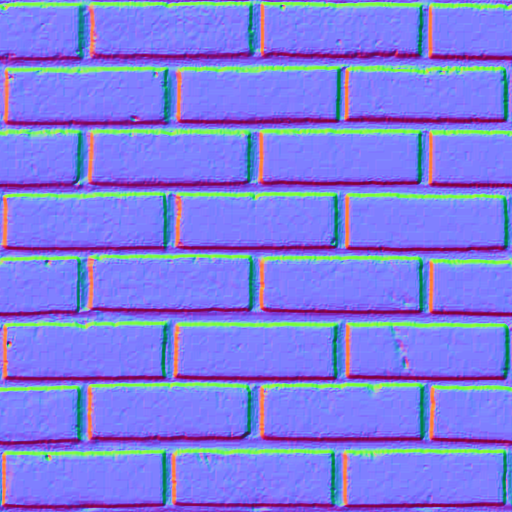
\includegraphics[width=0.3\textwidth]{figures/assignment7/BrickNormalMap.png}}
    \hfill
    \subcaptionbox{Copper \cite{texture-copper}}{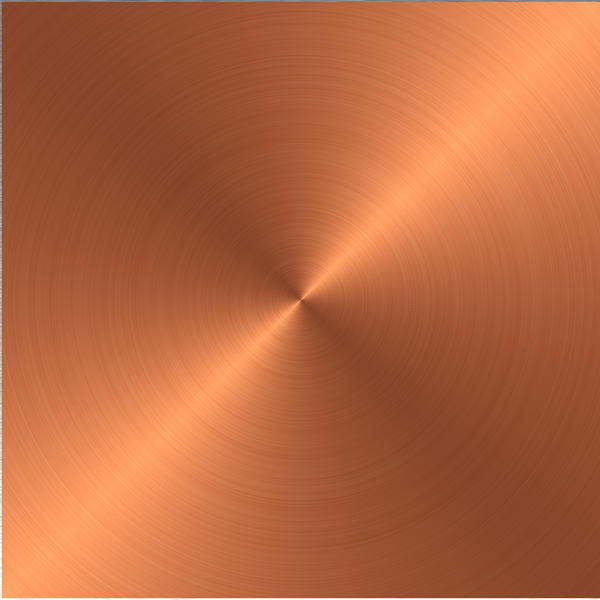
\includegraphics[width=0.3\textwidth]{figures/assignment7/copper.jpg}}
    
    \break
    
    \subcaptionbox{Gold \cite{texture-gold}}{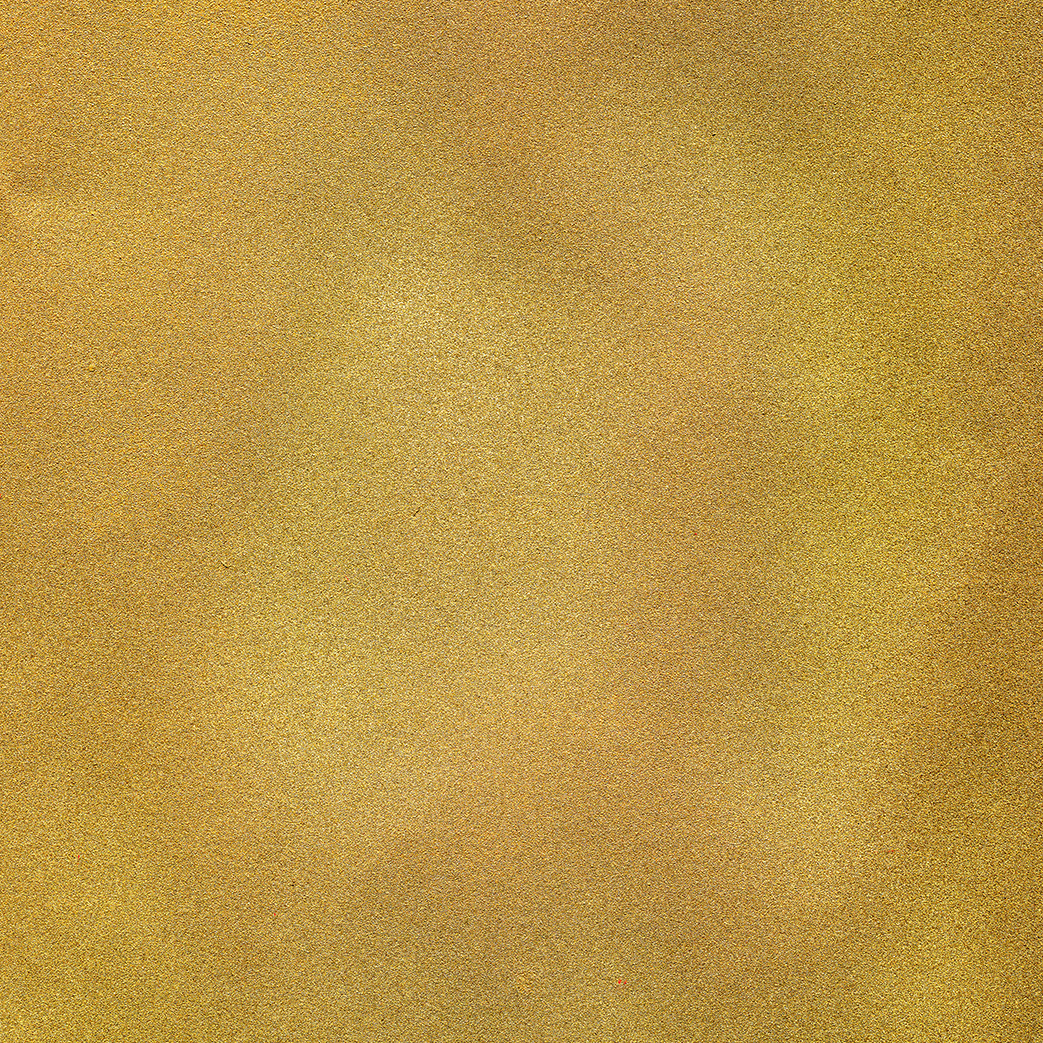
\includegraphics[width=0.3\textwidth]{figures/assignment7/gold.jpg}}
    \hfill
    \subcaptionbox{Plastic \cite{texture-plastic}}{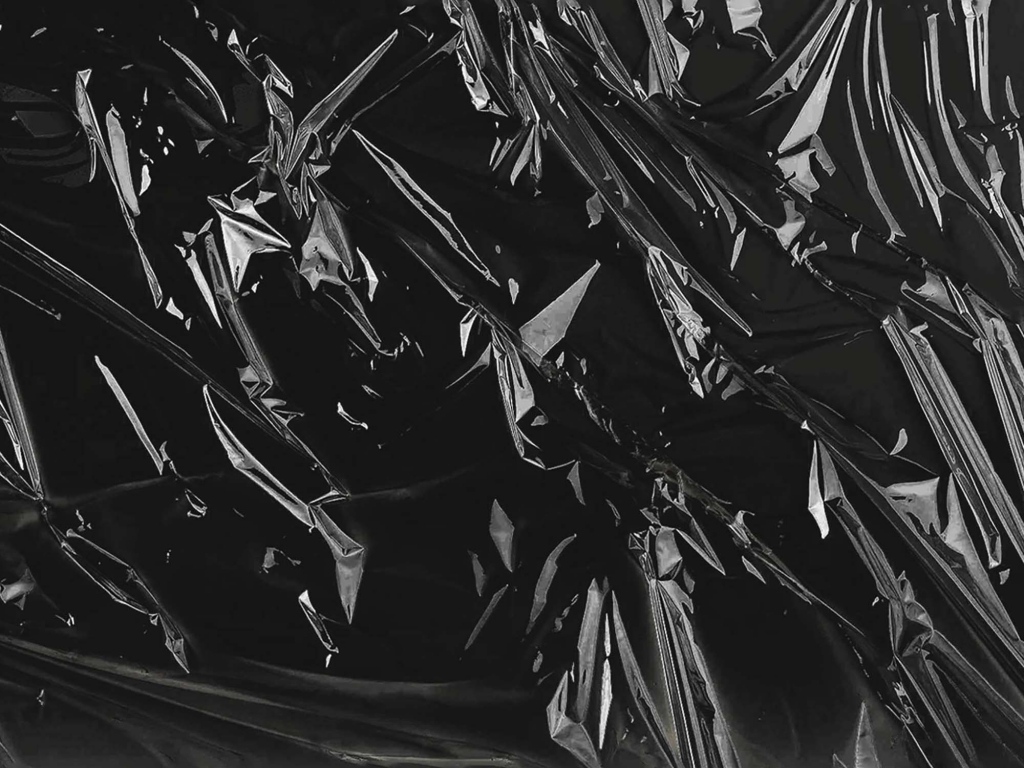
\includegraphics[width=0.3\textwidth]{figures/assignment7/plastic-2.jpg}}
    \hfill
    \subcaptionbox{Wood \cite{texture-wood}}{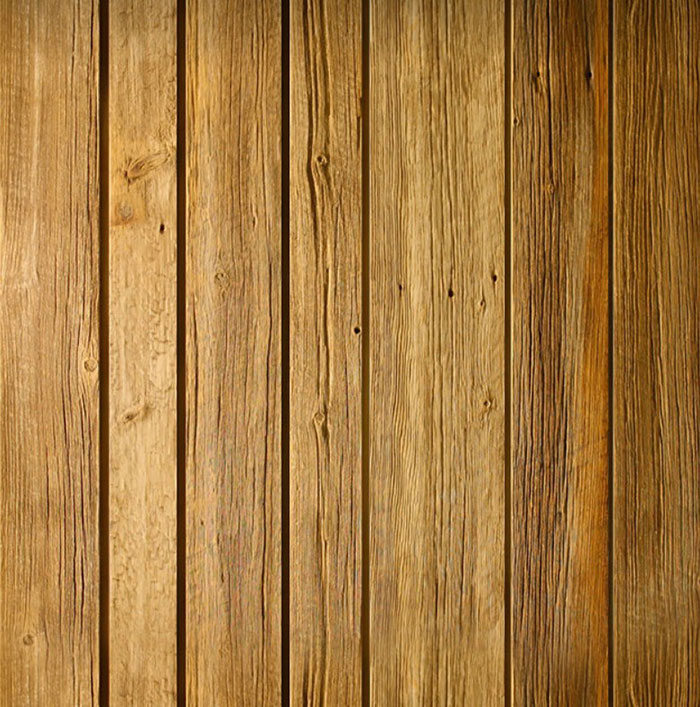
\includegraphics[width=0.3\textwidth]{figures/assignment7/wood.jpg}}
    
    \caption{Textures used in the program}
\end{figure}

\end{document}